\documentclass{article}
\usepackage{tikz}
\usepackage{xcolor}

\definecolor{myblue}{RGB}{54,106,146}
\definecolor{bggray}{RGB}{240,240,240}

\begin{document}

\begin{center}
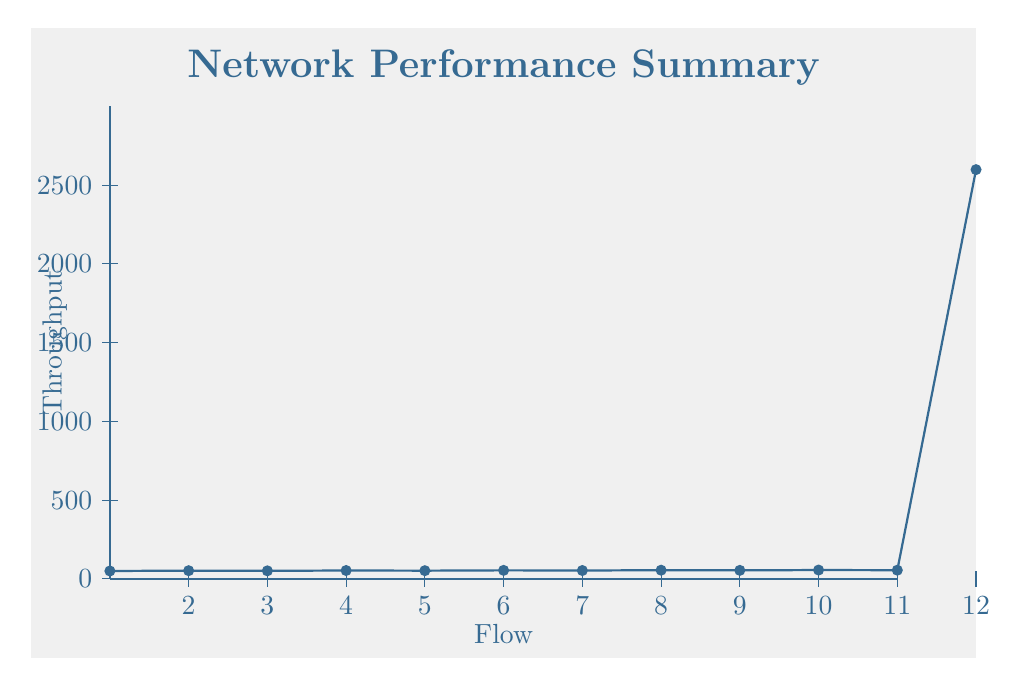
\begin{tikzpicture}

% Background
\fill[bggray] (0,0) rectangle (12,8);

% Axes
\draw[thick, myblue] (1,1) -- (1,7); % Y-axis
\draw[thick, myblue] (1,1) -- (11,1); % X-axis

% Title
\node[text=myblue, font=\Large\bfseries] at (6,7.5) {Network Performance Summary};

% Axis Labels
\node[text=myblue] at (6,0.3) {Flow};
\node[rotate=90, text=myblue] at (0.3,4) {Throughput};

% Y-axis ticks
\foreach \y/\val in {1/0,2/500,3/1000,4/1500,5/2000,6/2500} {
    \draw[myblue] (0.9,\y) -- (1.1,\y);
    \node[left, text=myblue] at (0.9,\y) {\val};
}

% X-axis ticks
\foreach \x in {2,3,4,5,6,7,8,9,10,11,12} {
    \draw[myblue] (\x,0.9) -- (\x,1.1);
    \node[below, text=myblue] at (\x,0.9) {\x};
}

% Data points (scaled)
\def\scale{0.002}

\foreach \x/\y in {
1/50,2/52,3/51,4/53,5/52,6/54,
7/53,8/55,9/54,10/56,11/55,12/2600} {
    \fill[myblue] (\x,{1 + \y*\scale}) circle (2pt);
}

% Connecting lines
\draw[myblue, thick]
(1,{1+50*\scale}) --
(2,{1+52*\scale}) --
(3,{1+51*\scale}) --
(4,{1+53*\scale}) --
(5,{1+52*\scale}) --
(6,{1+54*\scale}) --
(7,{1+53*\scale}) --
(8,{1+55*\scale}) --
(9,{1+54*\scale}) --
(10,{1+56*\scale}) --
(11,{1+55*\scale}) --
(12,{1+2600*\scale});

\end{tikzpicture}
\end{center}

\end{document}